\chapter{The '3' on THREE Overprint}

\ph[width = .50\textwidth]{../cape-of-good-hope/images/3-Sheet-Reconstruction.jpg}{
'3' on three sheet reconstruction
Reconstruction of sheet based on information from surviving blocks and strips.
}


THE "3" ON THREE PENCE PALE DULL ROSE OVERPRINT
(Issued August 1880)

The new Three pence stamps received from England had been in issue for 
two or three days when the Postmaster General reported that his previously 
expressed fears, as to the confusion with the One Penny stamps had
been found to be true and that inconvenience and difficulties were 
already being experienced.



He requested that immediate steps be taken to instruct the 
Government printers to surcharge all the Three Pence stamps 
in stock with a distinctive mark which he suggested should be 
a large "3".

\ph[width = .60\textwidth]{../cape-of-good-hope/images/3-ON-THREE-IMAGES/narrow-3-block.jpg}{
Block of four proving that the stamps were printed at least on two rows.}

Arrangements were made with Messrs. Saul Solomon \& Co. and 
the surcharging is officially recorded as having commenced 
on the 26th July 1880.

It is believed that the surcharge was applied to 60 stamps (one pane) 
at each operation. Owing to the insufficiency of figures of the same 
font the work was carried out using a broad "3" and a narrow "3".
Block of four proving that the stamps were printed at least on two rows.
'3' on three error

Strip of three with middle stamp missing the '3'


\ph[width = .30\textwidth]{../cape-of-good-hope/images/3-ON-THREE-IMAGES/3-on-three-omitted.jpg}{ }






There is nothing in the records to indicate the arrangement of the types. 
But based on surviving blocks it is probable that the first eight rows consisted
of the broad  
and the last two rows of the narrow 3. Based on the block of four illusttarted 
here at least two rows
 consisted of the narrow '3'. The strip of three illustrated also here 
 shows the middle stamp 
 missing the overprint confirming that the missing '3'must have existed 
 on the 9th row., 
 these stamps must have existed on the ninth row, although their 
 position is conjectural.{{footnote: 1, 2,3,4}}.

The fact that there were two narrow rows printed can be deduced from 
blocks of three that exist (see adjacent photograph).(Allis states that 
there were nine rows of the broad "3" and one of the narrow "3". 
This is incorrect as can be deduced from the block of  four shown here).

Many other varieties exist.

\begin{marginfigure}
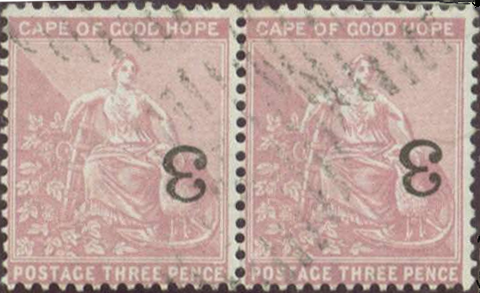
\includegraphics[width=0.95\textwidth]{../cape-of-good-hope/images/3-ON-THREE-IMAGES/3-pair-inverted.png}
\end{marginfigure}


\section{References}


1 Allis states that there were nine rows of the broad "3" and one of 
the narrow "3". This is incorrect as can be deduced from the block of  
four shown on the next page of this exhibit.


2 Robson Lowe states that the "forme" for printing the surcharge was 
probably made of 48 of Type I and 10 of Type II, two having  the surcharge omitted. 
The sixth stamp of the ninth row was definitely without a surcharge. 
Either the second, third, fourth or fifth  were without a surcharge.


3 Jurgens reports having seen the two types se-tenant horizontally. This 
was probably a replacement when the printers became  aware of the problem.


4 Lowe states that stamps surcharge "3" in manuscript are known. They may 
be attempts to correct the stamps with overprint omitted. 

                    